\documentclass[12pt,a4paper]{report}
\usepackage[utf8]{inputenc}

\usepackage{ucs}
\usepackage{amsmath}
\usepackage{amsfonts}
\usepackage{amssymb}
\usepackage{listings}
\usepackage{color}
\usepackage{graphicx}
\pagestyle{headings}
\author{Frédéric BOLLON}
\title{Fredistrano v1.0\\Documentation\\}
\begin{document}
	% FIXME F2: update documentation 
\maketitle
\tableofcontents

\chapter{Introduction}
Fredistrano is a deployment tool for PHP web applications. It automates the export of your sources from a subversion repository and synchronizes them with the content of a target directory. Several manual tasks are also handled directly by the application during the deployment: renaming of configuration files, modifying permissions... Fredistrano is inspired from the smart Capistrano project.\\

From a technical perspective, this application has been written in PHP with the cakePHP framework. Fredistrano both supports Windows/Linux environment. Concerning Windows, Fredistrano requires the installation of Cygwin in order to use the rsync command.\\

Special thanks to Aurélien Millet and euphrate\_ylb for their help in this project.

\chapter{Requirements}
Fredistrano must be installed on a Apache Web server hosted \textbf{indifferently} under Linux or Windows.
\paragraph*{Common to all OS}
\begin{itemize}
\item 
A Php project "versioned" with Subversion
\item 
A Php web hosting with the safe\_mode set to Off and mod\_rewrite activated\\\\
\begin{small}\textit{If mod\_rewrite is not working you will need to remove the comment from app/config/core.php\\
      a. Around line 59: Configure::write('App.baseUrl', env('SCRIPT\_NAME'));\\
      b. Then access using http://www.example.com/my\_directory/index.php/pages to verify installation is working}\end{small}
\end{itemize}

\paragraph*{Windows only}
\begin{itemize}
\item
For deployment on windows servers, you need to install cygwin with packages rsync, perl and subversion.

\end{itemize}

\chapter{Installation}
\begin{itemize}
\item Download the lastest version of Fredistrano on\\ http://code.google.com/p/fredistrano/downloads/list
\item Untar the archive at the root of your web server or in a directory of your choice \: \\
tar xzvf fredistrano\_x.x.tar.gz \\
\item Give writable permission to temporaries directories (only on linux servers).\\
\begin{verbatim}

chmod -R 777 app/tmp/ files/

\end{verbatim}

\item Create the database with the sql script in\\ /app/config/sql/fredistrano.sql\\
\item Create files app/config/config.php et app/config/database.php with the help of config.prd.php and database.prd.php\newpage

\item Configure app/config/database.php following your database\\\\example :\\

%---------------------------------------------------------------
\definecolor{lbcolor}{rgb}{0.9,0.9,0.9}
\lstset{language=Php}
\lstset{commentstyle=\textit}
%\lstset{backgroundcolor=lbcolor,framerulecolor=}
\lstset{backgroundcolor=\color{lbcolor},rulecolor=}
\lstset{literate={<=}{{$\le$}}{2}}
%\color{yellow}

\lstset{literate={=}{{$\leftarrow$}}{1}{<=}{{$\le$}}{2}{&&}{{$\cap$}}{2}}
\begin{lstlisting}[frame=tb]{}
var $default = array(
	'driver' => 'mysql',
	'persistent' => false,
	'host' => 'localhost',
	'login' => 'usermysql',
	'password' => 'password',
	'database' => 'fredistrano'
	'encoding' => 'utf8'
);
\end{lstlisting}
%---------------------------------------------------------------

\item A user "admin" with password "pass" is created by the sql script, don't forget to change password in Administration/users.
If you create a new user, you need to affect if the group "admin".
\textbf{Do not delete the user "admin" before creating a new user for the group "admin".}

\end{itemize}

\chapter{Usage}
\section{Setting up your project}\label{precimportantes}
Before being able to deploy your project with fredistrano, you must set it up according to the following recommandations :\\
\begin{itemize}
\item Your project must be versionned with subversion.\\
\item If the content of some files differs between the deveploment environment and the production one, these files shouldn't be added to subversion but only copies with an extension like '.dev.xxx' et '.prd.xxx':\\
For example, if the application requires a database.php file where connection parameters are defined, you won't add directly this file to subversion. Instead, you will add two other versions, one for each environment, nammed database.dev.php and database.prd.php.\\ 
During the deployment, whatever the extension is, all 'prd.xxx' files will be deployed (not 'dev.xxx' ones) and renamed in '.xxx'.
\item A 'deploy.php' file must be created at the application root. This files contains application specific deployment parameters such as a list of files and folders that shouldn't be synchronized, a list of writable directories... Notice that this file won't be deployed in your production environment. Here is an example of deploy.php :\\

%---------------------------------------------------------------
\definecolor{lbcolor}{rgb}{0.9,0.9,0.9}
\lstset{language=Php}
\lstset{breaklines=true}
\lstset{tabsize=2}
\lstset{morecomment=[l]{//}}
\lstset{commentstyle=\textit}
\lstset{backgroundcolor=\color{lbcolor},rulecolor=}
\begin{lstlisting}[frame=tb]{}
	<?php
	 class DEPLOY_CONFIG {

		// Default deployment options for the current project
		// these options could be modified during the deployment process in standard mode
		// in fast mode these options will be used
	 	var $options = array(
	 		'export' 		=> array(),
	 		'synchronize'	=> array(
	 		 	'runBeforeScript'		=> 	false, 		//enable custom script before deployement 
	 			'backup'				=> 	false 		//enable backup functionality
	 		),
	 		'finalize'		=> array(
		 		'renamePrdFile' 		=> 	false,		//enable renaming .prd.xxx files
				'changeFileMode' 		=> 	false,		//enable updating file mode
				'giveWriteMode'			=> 	false,		//enable updating write mode on directories defined in $writable (in this file)
	 			'runAfterScript'		=> 	false		//enable custom script at the end of the deployement process
	 		)
	 	);

	 	// path of yours custom scripts to execute at the beginning/end of the deployment process
		// if yours scripts are located in a directory named ".fredistrano" at the root of your project enter only the name of your script to execute
	 	var $scripts = array(
	 		'before' 	=>		'/path/to/file', 
	 		'after' 	=>		'/path/to/file' 
	 	);

		// List of directories and files to exclude during the deployemnt process on the production server
		var $exclude = array (
			'app/tmp/logs/*',
			'app/tmp/sessions/*',
			'app/tmp/tests/*',
			'app/config/database.php',
			'app/config/config.php',
			'app/webroot/files/*',
			'files/logs/*',
			'files/tmp/*'
		);

		// Directories list on which the write permission will applied during the finalization step of the deployment process	
		// log, cache, upload directories, etc...
		var $writable = array (
			'app/tmp',
			'files/backup',
			'files/logs'
		);

	 }// DEPLOY_CONFIG
	?>
\end{lstlisting}
%---------------------------------------------------------------

\end{itemize}
\newpage

\section{Deployment steps}

\subsection{Adding a new project}

To deploy a PHP web application with Fredistrano, the first step is to create a new project.\\

\begin{enumerate}
\item Click on the "Projects" toggle (Top of your screen)
\item Click on the "Add a new project" link
\item Fill out the form as follow:\\

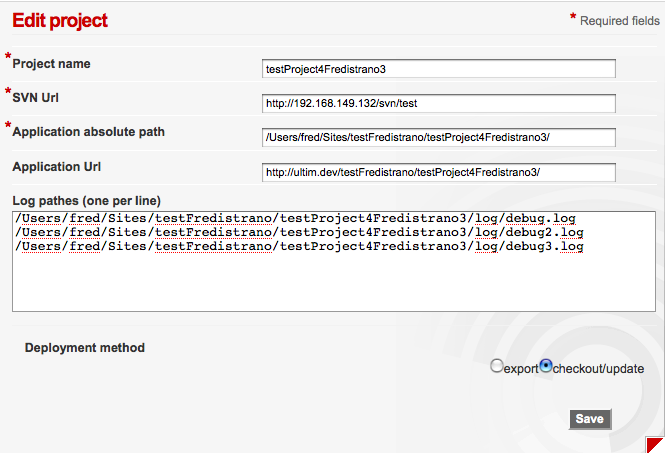
\includegraphics[width=1\textwidth]{doc_fredistrano1.png} 


\begin{list}{- Field:}{}
\item \textbf{"Project name"} : Is used to identify the project. It will also be used as a diretory name for temporary copy during the deployment. Do not use special characters.
\item \textbf{"SVN Url"} :  Url of the SVN repository of the project that should be deployed (eg. : "http://svn.mondomain.com/monProjet/trunk").
\item \textbf{"Application Url"} : Won't be used by Fredistrano. Juste a simple reminder.
\item \textbf{"Absolute path"} :  Absolute path of the target folder where the application should be deployed\\Example for a Windows server (located on the server) : D:\textbackslash www\textbackslash html\textbackslash myProject \\Example on a Linux server : /var/www/html/monProjet or /home/monUser/monDomain.com.
\item \textbf{"Log pathes"} : Pathes of files that you want to access with the log viewer, one path per line.
\end{list}
\end{enumerate}

\subsection{Project deployment}
\begin{enumerate}
\item Display the details of the project that should be deployed.
\item Click on "Deploy project".
\item Specify the revision number. If empty, Fredistrano will checkout the latest revision of the repository.
\item In the case of a private Suversion project protected by login/password, you may specify your credentials at this step. If all your projects are using the same credentials, you may specify them in the file \textit{app/config/config.php}.
\item Click on "Step 1 SVN export". An svn export is executed and the result is displayed in the console located at the bottom (\textit{output console}) "Fredistrano/files/tmp/nomduprojet/tempDir".
\item For the next step, if "simulate" is checked, the rsync command will only be simualted and its  result may be seen in the output console.
\item Click on "Step 2 synchronize".
\item A backup is preformed in "Fredistrano/files/backup/projectName". The rsync command is executed between "Fredistrano/files/tmp/projectName/tempDir" and "projectName".
\item Finally, as the last step, three options may be overridden: 1. renaming of '.prd.' files, 2. force files and folders permissions, 3. set write privileges on special folders . The inial values depend on the content of your config.php file.
\item Click on "Step 3 finalize" and your done!
\end{enumerate}

\subsection{Project deployment fast mode}
\begin{enumerate}
\item Display the details of the project that should be deployed.
\item Click on the "switch deployment mode" link to change the button "Deploy" to "Fast deploy"
\item All the steps will be execute with standard options (renaming prd files, changing file mode on modified files only, giving write mode). 
\end{enumerate}

\section{Deployment logs}
You can access the deployment history from the details page of each project by clicking on the link "view deployment history". A rss feed of deployment history is available in the menu on this page. It is possible to disable rss feeds in /app/config/config.php 

\section{Logs viewer}
Click on the "Logs" tab to use the log viewer, with this feature you can diplay the content of the logs files defined in the project details
\chapter{Related links}
You will find in the following 
\begin{itemize}
\item An example of web host that satisfy the requirements of Fredistrano \\ http://www.fbollon.net/node/12 \\
\item A quick explanation on how to use Subversion \\ http://www.fbollon.net/node/65 \\
\item The official support forum of Fredistrano \\ http://www.fbollon.net/forum/23
\end{itemize}


\end{document}